
\renewcommand{\summarizedlecture}{7 }

%
%
%

\begin{frame}{Lecture \summarizedlecture revision}

In the last lecture:\\

\begin{itemize}

   \item We completed the study of {\bf Maxwell's eqs. in materials (for static fields)}
             and emphasized the analogies between electrostatics and magnetostatics.

   \vspace{0.2cm}

   \item We discussed the magnetic properties of materials
             ({\bf diamagnetism}, {\bf paramagnetism} and {\bf ferromagnetism})
             and developed arguments to understand the physical origins.

   \vspace{0.2cm}

   \item We found out how to {\bf extend Maxwell's eqs. in vacuum}
             in the case of {\bf time-dependent fields}.

\end{itemize}

\end{frame}

%
%
%

\begin{frame}{Lecture \summarizedlecture revision (Magnetic moment / magnetization)}

\begin{columns}
  \begin{column}{0.25\textwidth}
    \begin{center}
      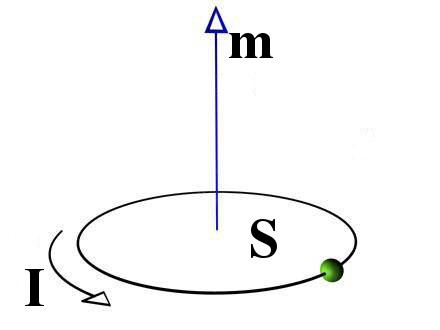
\includegraphics[width=0.95\textwidth]{./images/schematics/magnetic_dipole_moment_00.jpg}\\
    \end{center}
  \end{column}
  \begin{column}{0.70\textwidth}
    We defined the {\bf magnetic dipole moment} $\vec{m}$ as:
   \begin{equation*}
     \vec{m} = I \vec{S}
   \end{equation*}
  \end{column}
\end{columns}

\vspace{0.2cm}

An external magnetic field $\vec{B}$ exerts a torque $\vec{T}$ on a magnetic dipole $\vec{m}$ which is given by:
\begin{equation*}
  \vec{T} = \vec{m} \times \vec{B}
\end{equation*}

This will tend to {\bf align} the previously randomised {\bf magnetic moments}
and {\bf create magnetisation at a macroscopic level}.\\
\vspace{0.2cm}

We define {\bf magnetisation} $\vec{M}$ as the amount of {\bf magnetic dipole moment per unit volume}.

\end{frame}

%
%
%

\begin{frame}{Lecture \summarizedlecture revision (Magnetization-induced currents)}

The {\bf magnetisation induces surface and volume currents}.\\
\vspace{0.3cm}
We can easily be convinced, although we will not show it mathematically,
that the {\bf density of the surface current} is:
\begin{equation*}
  j_{m}^{surf} = \vec{M} \times \hat{n}
\end{equation*}

\vspace{0.1cm}

whereas the {\bf density of the volume current} is:
\begin{equation*}
  j_{m}^{vol} = \vec{\nabla} \times \vec{M}
\end{equation*}

\begin{center}
  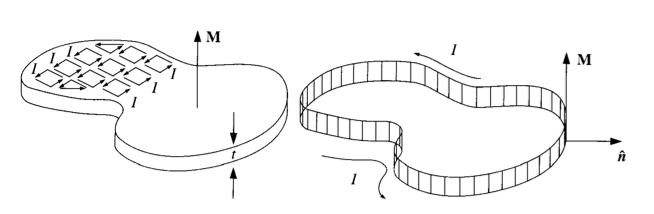
\includegraphics[width=0.98\textwidth]{./images/schematics/magnetization_currents_01.png}\\
\end{center}

\end{frame}

%
%
%

\begin{frame}{Lecture \summarizedlecture revision (Ampere's law in materials)}

We started from Ampere's law in vacuum:
\begin{equation*}
  \vec{\nabla} \times \vec{B} = \mu_0 \vec{j}
\end{equation*}
By writing the total current density $\vec{j}$ as the vector sum of the free ($\vec{j}_{f}$)
and magnetization ($\vec{j}_{m}$) current densities,
and expressing $\vec{j}_{m}$ in terms of the
magnetization field $\vec{M}$ ($\displaystyle \vec{j}_{m} = \vec{\nabla} \times \vec{M}$),
we finally wrote Ampere's law as:
\begin{equation*}
  \vec{\nabla} \times \Big( \frac{\vec{B}}{\mu_0} - \vec{M} \Big) = \vec{j}_{f}
\end{equation*}

We defined the {\bf magnetic field strength} or {\bf magnetic field intensity} $\vec{H}$ as:
\begin{equation*}
  \vec{H} = \frac{\vec{B}}{\mu_0} - \vec{M}
\end{equation*}
In SI, the quantity $\displaystyle \vec{H} = \frac{\vec{B}}{\mu_0} - \vec{M}$ has {\bf units of A/m}.\\

\end{frame}

%
%
%

\begin{frame}{Lecture \summarizedlecture revision (Linear materials)}

Ampere's law in materials is:
$\displaystyle \vec{\nabla} \times \Big( \frac{\vec{B}}{\mu_0} - \vec{M} \Big) = \mu_0 \vec{j}_{f}$\\
\vspace{0.1cm}

If the analogy with electrostatics was exact,
we would write $\vec{M}$ in terms of $\vec{B}$.
However, this is where the analogy breaks.
Instead we typically write:
\begin{equation*}
{\color{magenta}
  \vec{M} = \chi_{m} \vec{H}
}
\end{equation*}
where  $\chi_m$ is the {\bf magnetic susceptibility}.
For {\bf linear materials}, $\chi_m$ is a constant independent of the value of $\vec{H}$.
Expressing $\vec{B}$ in terms of $\vec{H}$:
\begin{equation*}
  \vec{H} = \frac{\vec{B}}{\mu_0} - \vec{M} \Rightarrow
  \vec{B} = \mu_0 \Big( \vec{H} + \vec{M} \Big) \xRightarrow{\vec{M} = \chi_{m} \vec{H}}
  \vec{B} = \Big(1 + \chi_{m} \Big) \mu_0  \vec{H} \Rightarrow
\end{equation*}
\begin{equation*}
  \vec{B} = \mu_r \mu_0 \vec{H} \Rightarrow
  {\color{magenta}
    \vec{B} = \mu \vec{H}
  }
\end{equation*}
where $\mu_r = 1+\chi_{\mu}$
is the {\bf relative permeability} (dimensionless) and
$\mu = \mu_r  \mu_0$ is the {\bf permeability} of the material
(SI unit: $V \cdot s \cdot  A^{-1} \cdot m^{-1}$).\\

\end{frame}

%
%
%

\begin{frame}{Lecture \summarizedlecture revision (Correspondence between quantities)}

{
\setlength{\extrarowheight}{8pt}
\setlength{\arraycolsep}{5pt}

\begin{center}
  \begin{table}[H]
    \begin{tabular}{c|c||c|c}
      \hline
      \multicolumn{2}{c||}{\bf Electrostatics} &
      \multicolumn{2}{c}  {\bf Magnetostatics} \\
      \hline
         {\scriptsize electric dipole moment} &
         $\vec{p} = q \vec{d}$ &
         $\vec{m} = I \vec{S}$ &
         {\scriptsize magnetic dipole moment} \\
      \hline
         {\scriptsize torque within $\vec{E}$ field} &
         $\vec{T} = \vec{p} \times \vec{E}$ &
         $\vec{T} = \vec{m} \times \vec{B}$ &
         {\scriptsize torque within a $\vec{B}$ field} \\
      \hline
         {\scriptsize polarization} &
         $\vec{P}  = \frac{(e.d.m)}{volume}$ &
         $\vec{M} = \frac{(m.d.m)}{volume}$ &
         {\scriptsize magnetization} \\
      \hline
         {\scriptsize surface charge density} &
         $\sigma_{P} = \vec{P} \cdot \hat{n}$ &
         $j_{m}^{surf} = \vec{M} \times \hat{n}$ &
         {\scriptsize surface current density} \\
      \hline
         {\scriptsize volume charge density} &
         $\rho_{P} = - \vec{\nabla} \cdot \vec{P}$ &
         $j_{m}^{vol} = \vec{\nabla} \times \vec{M}$ &
         {\scriptsize volume current density} \\
      \hline
         {\scriptsize electric displacement} &
         $\vec{D} = \epsilon_0 \vec{E} + \vec{P}$ &
         $\vec{H} = \frac{\vec{B}}{\mu_0} - \vec{M}$ &
         {\scriptsize magnetizing field} \\
      \hline
         \multirow{2}{*}{\scriptsize Gauss' law in materials} &
         $\vec{\nabla} \cdot \vec{D} = \rho_{f}$ &
         $\vec{\nabla} \times \vec{H} = \vec{j}_{f}$ &
         \multirow{2}{*}{\scriptsize Ampere's law in materials} \\
      \hhline{~--~}
         &
         $\oint_{S} \vec{D} \cdot d\vec{S} = Q_{f}$ &
         $\oint_{L} \vec{H} \cdot d\vec{\ell} = I_{f}$ &
         \\
      \hline
    \end{tabular}
  \end{table}
\end{center}
}

\end{frame}

%
%
%

\begin{frame}{Lecture \summarizedlecture revision (Magnetic properties of materials)}

\begin{itemize}

\item We also discussed the {\bf magnetic properties of materials}
          and developed (classical) arguments to understand the {\bf physical origins}.

\item The material which has the {\bf most striking and well known
          magnetic properties is iron (Fe).}

     \begin{itemize}
            \item Nickel (Ni), Cobalt (Co), Gadolinium (Gd) and Dysprosium (Dy) behave similarly.
                      We call these materials {\bf \color{magenta} ferromagnets}.
            \item Not only these materials can have a significant magnetisation when inside an
                      external magnetic field, they also {\bf retain their magnetisation in the absence
                      of an external magnetic field.}
     \end{itemize}

\item But {\bf other substances get magnetised too} (water, wood, frogs,...)

     \begin{itemize}
             \item The magnetic effects for these materials are {\bf very very weak!}
             \item Moreover, water, wood, and frogs {\bf do not remain magnetized} once the external
                       magnetic field is removed.
             \item In a presense of an external magnetic field these substances can be magnetised
                       either in the direction of the field ({\color{magenta} {\bf paramagnetic}} substances),
                       or opposite to it ({\color{magenta} {\bf diamagnetic}} substances).
     \end{itemize}

\end{itemize}

\end{frame}

%
%
%

\begin{frame}{Lecture \summarizedlecture revision (Maxwell's eqs. for the static case)}

{\small

\begin{center}
{
  \begin{table}[H]
    \begin{tabular}{|l|c|c|}
      \hline
        \multicolumn{3}{|l|} {
          {\color{magenta}
           {\bf Static case in vacuum}
          }
        }\\
      \hline
      {\bf Gauss's law} &
        $\displaystyle \oint \vec{E} \cdot d\vec{S} = \frac{1}{\epsilon_0} \int \rho d\tau$ &
        $\displaystyle \vec{\nabla} \cdot \vec{E} = \frac{\rho}{\epsilon_0}$ \\

      {\bf Circuital law} &
        $\displaystyle \oint \vec{E} \cdot d\vec{\ell} = 0$ &
        $\displaystyle \vec{\nabla} \times \vec{E} = 0$ \\

      {\bf Gauss's law} (magn.) &
        $\displaystyle \oint \vec{B} \cdot d\vec{S} = 0$ &
        $\displaystyle \vec{\nabla} \cdot \vec{B} = 0$ \\

      {\bf Ampere's law} &
        $\displaystyle \oint \vec{B} \cdot d\vec{\ell} = \mu_{0} \int \vec{j} \cdot d\vec{S}$ &
        $\displaystyle \vec{\nabla} \times \vec{B} = \mu_{0} \vec{j}$ \\

      \hline
    \end{tabular}
  \end{table}
}
\end{center}

\begin{center}
{
  \begin{table}[H]
    \begin{tabular}{|l|c|c|}
      \hline
        \multicolumn{3}{|l|} {
          {\color{magenta}
           {\bf Static case within materials}
          }
        }\\
      \hline
      {\bf Gauss's law} &
        $\displaystyle \oint \vec{D} \cdot d\vec{S} =  \int \rho_{f} d\tau$ &
        $\displaystyle \vec{\nabla} \cdot \vec{D} = \rho_{f}$ \\

      {\bf Circuital law} &
        $\displaystyle \oint \vec{E} \cdot d\vec{\ell} = 0$ &
        $\displaystyle \vec{\nabla} \times \vec{E} = 0$ \\

      {\bf Gauss's law} (magn.) &
        $\displaystyle \oint \vec{B} \cdot d\vec{S} = 0$ &
        $\displaystyle \vec{\nabla} \cdot \vec{B} = 0$ \\

      {\bf Ampere's law} &
        $\displaystyle \oint \vec{H} \cdot d\vec{\ell} =  \int \vec{j}_{f} \cdot d\vec{S}$ &
        $\displaystyle \vec{\nabla} \times \vec{H} = \vec{j}_{f}$ \\
      \hline
    \end{tabular}
  \end{table}
}
\end{center}
}

\end{frame}
